\RequirePackage{fix-cm}
\documentclass[a4paper,ngerman]{scrartcl}

\usepackage[utf8]{inputenc}
\usepackage{cmbright}
\usepackage[T1]{fontenc}
\usepackage{babel}
\DeclareUnicodeCharacter{FEFF}{}

\usepackage{paralist}	
\usepackage{geometry}	
\usepackage{tabularx}		
\usepackage{listings} 
\usepackage{datetime} 
\usepackage{graphicx}
\usepackage{enumitem}
\usepackage{booktabs}
\usepackage{multirow}
\usepackage{newunicodechar} 

\usepackage{color}
\usepackage{varioref} 
\usepackage[colorlinks=false, pdfborder={0 0 0}]{hyperref} 
\usepackage{cleveref} 

\setcounter{secnumdepth}{2} 
  
\definecolor{bluekeywords}{rgb}{0,0,1}
\definecolor{greencomments}{rgb}{0,0.5,0}
\definecolor{redstrings}{rgb}{0.64,0.08,0.08}
\definecolor{xmlcomments}{rgb}{0.5,0.5,0.5}
\definecolor{types}{rgb}{0.17,0.57,0.68}

\usepackage{listings}
\lstset{language=[Sharp]C,
	captionpos=b,
	showspaces=false,
	showtabs=false,
	breaklines=true,
	showstringspaces=false,
	breakatwhitespace=true,
	escapeinside={(*@}{@*)},
	commentstyle=\color{greencomments},
	morekeywords={partial, var, value, get, set, namespace},
	keywordstyle=\color{bluekeywords},
	stringstyle=\color{redstrings},
	basicstyle=\ttfamily\small,
	extendedchars=\true,
}

\begin{document}
\title{Amazing Race}
\subtitle{MOC5-Projekt}
\author{Stefan Kert}
\date{\today}
\maketitle
\section{Allgemeines}
Die Plattform, welche für die Projektarbeit ausgewählt wurde, ist Windows Phone 8.1. Es gibt bei der Version 8.1 der Plattform zahlreiche Vorteile, wie zum Beispiel eine bessere Unterstützung des .Net Frameworks und im Allgemeinen ist es zukunftsorientierter gestaltet. Als IDE wurde Visual Studio 2015 in der Enterprise Version verwendet und getestet wurde die App auf einem Emulator mit WP 8.1 und einem Emulator mit WP 10. 

\section{Lösungsidee}
Bei der Lösung wird auf eine möglichst gute Trennung der einzelnen Aspkete geachtet. Es wird dabei das in der .NET Programmierungsumgebung etablierte MVVM Pattern angewandt verwendet. Durch dieses wird eine gute Trennung zwischen View und Logik gewährleistet. Weiters wird eine eigene Klasse für die Interaktion mit dem Webservice implementiert. 


\subsection{Anwendungsstruktur}
Grundsätzlich besteht die \textit{AmazingRace}-App aus 3 Pages:
\begin{itemize}
	\item \textbf{LoginPage}: Hier erfolgt der Login. Falls die Zugangsdaten nicht erfolgreich sind, wird dem User eine entsprechende Fehlermeldung angezeigt.
	\item \textbf{RoutesPage}: Bietet eine Übersicht über alle verfügbaren Schnitzeljagd-Routen und die Möglichkeit, alle Routen zurückzusetzen. Diese Reset-Funktionalität wurde über einen AppBar-Button realisiert. Die verfügbaren Routen werden mit einem Icon in einer ListView angezeigt.
	\item \textbf{RouteDetailsPage}: Nachdem eine Route ausgewählt wurde, werden hier Details dazu angezeigt. Die Seite zeigt einerseits Titel und Hinweis des nächsten Checkpoints, und andererseits eine Karte, auf der dieser markiert ist. Außerdem wird die bereits zurückgelegte Route inkl. aller bisherigen Checkpoints auf der Karte eingezeichnet.
	
Außerdem kann der User über einen Button einen ContentDialog öffenen, indem die "`Secret"'-Passwortphrase für den nächsten Checkpoint eingetragen werden kann. Falls diese korrekt ist, werden sofort alle Details für den nächsten Checkpoint angezeigt.

Beim Abschluss einer Route (bzw. wenn der User zu einer Route navigiert, die bereits abgeschlossen ist) wird eine Erfolgsmeldung in Form eines MessageDialog eingeblendet und der User kann seinen zurückgelegten Weg nochmals auf der Karte betrachten.
\end{itemize}
\subsection{Implementierungsdetails}
\subsubsection{Architektur}
Die Anwendung setzt das für Windows-Anwendungen und -Apps typische MVVM-Muster um; das bedeutet, dass es zu jeder der drei in Abschnitt~\ref{cha:Anwendungsstruktur} beschriebenen Views ein entsprechendes ViewModel gibt. Dieses kennt die Views nicht, sondern bietet Datenkomponenten und Commands an, an die sich die View binden kann. Die Oberfläche bleibt dadurch austauschbar, ohne die Business Logic verändern zu müssen -- diese könnte ohne großen Aufwand z.B. auch für eine Windows-Desktopanwendung verwendet werden (Abb.~\ref{fig:arch}). 


\subsubsection{Webservice-Anbindung}
Um die Applikation Daten mit dem Webservice austauschen zu lassen, wurde ein einfacher Service-Proxy entwickelt, der über einen \textit{HttpClient} GET- und POST-Requests ausführen und die Rückgabedaten direkt auf die entsprechenden Objekte mappen kann (für das Mapping wurde die von Microsoft empfohlene Bibliothek JSON.NET verwendet). Die Klasse \textit{ServiceProxy}, die das Interface \textit{IServiceProxy} implementiert, stellt dazu komfortable Methoden zur Verfügung. 

Die Login-Funktionalität wurde zudem noch in eine Klasse gekapselt, die das Singleton-Pattern implementiert (\textit{LoginService}). Dies stellt sicher, dass jede Page den Login-Status sowie die Benutzerdaten verwenden kann -- sollte eine Page aufgerufen werden, ohne dass ein User eingeloggt ist, wird der Benutzer auf die Login-Page weitergeleitet.

\subsubsection{Lifecycle-Management}
Der Lifecycle von Windows Phone 8.1-Apps ist prinzipiell dem von WP8 sehr ähnlich, allerdings gibt es kein \textit{Application-Deactivated}-Event mehr -- in WP8.1 werden Apps nicht mehr deaktiviert oder beim Verlassen beendet, sondern in den \textit{Suspended}-Status versetzt. Trotzdem kann die App bei Speicherknappheit beendet werden, dies geschieht ohne weitere Warnung.

Es muss also bei jedem Übergang in den \textit{Suspended}-Zustand angenommen werden, dass die App terminiert werden könnte. Um den Zustand der App zu persistieren, exisitert ein dem von WP8 bekannten State-Dictionary ähnliches Konstrukt: das \textit{SessionState}-Dictionary in der Klasse \textit{SuspensionManager}, die zudem noch die Möglichkeit, den Zustand eines Frames zu persistieren, enthält. Diese Funktionalität wird benutzt, um den Login-Status der App beizubehalten und die Login-Seite falls nötig zu überspringen.


\newpage
\section{Testfälle und Screenshots}

\subsection{Login Fenster}

\begin{figure}[h]
\centering
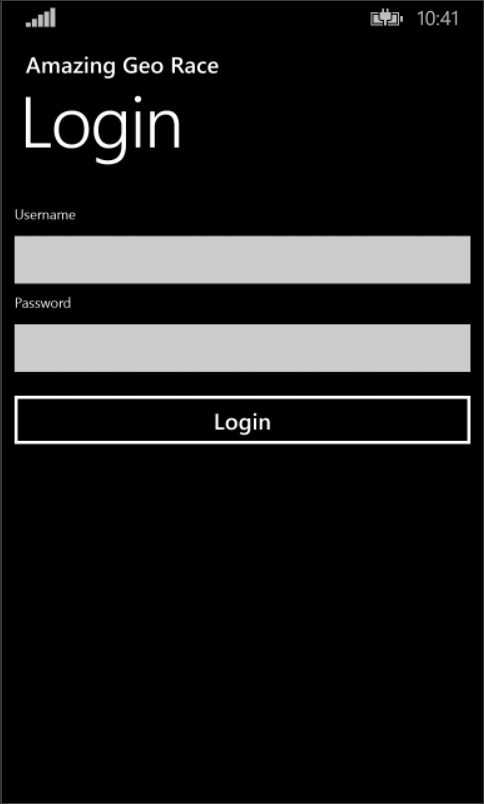
\includegraphics[width=.95\textwidth]{images/loginPage}
\caption{Grundfenster Login}
\end{figure}

\begin{figure}[h]
\centering
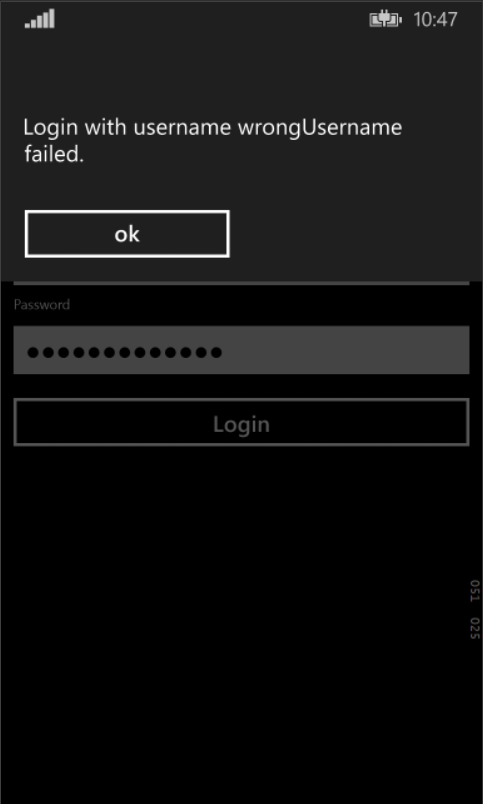
\includegraphics[width=.95\textwidth]{images/loginPage_Failed}
\caption{Feher beim Login}
\end{figure}

\subsection{Routenübersicht}

\begin{figure}[h]
\centering
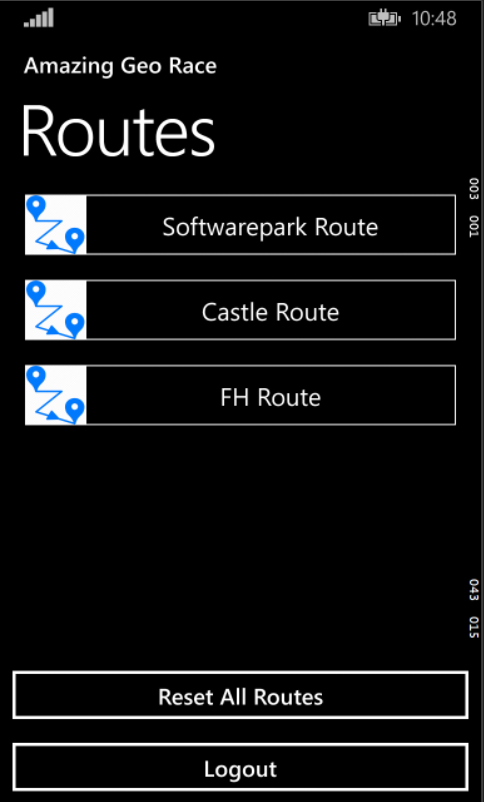
\includegraphics[width=.95\textwidth]{images/routePage}
\caption{Übersicht Routen}
\end{figure}

\begin{figure}[h]
\centering
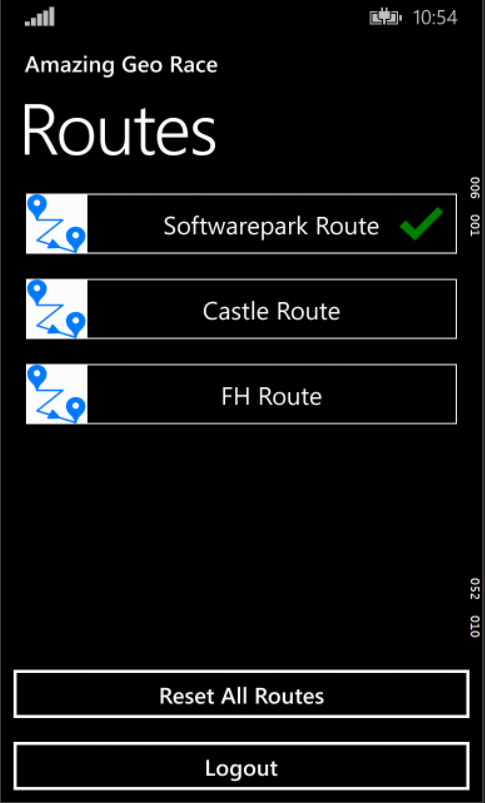
\includegraphics[width=.95\textwidth]{images/routePage_SucceededRoute}
\caption{Eine Route erfolgreich abgeschlossen}
\end{figure}
\begin{figure}[h]
\centering
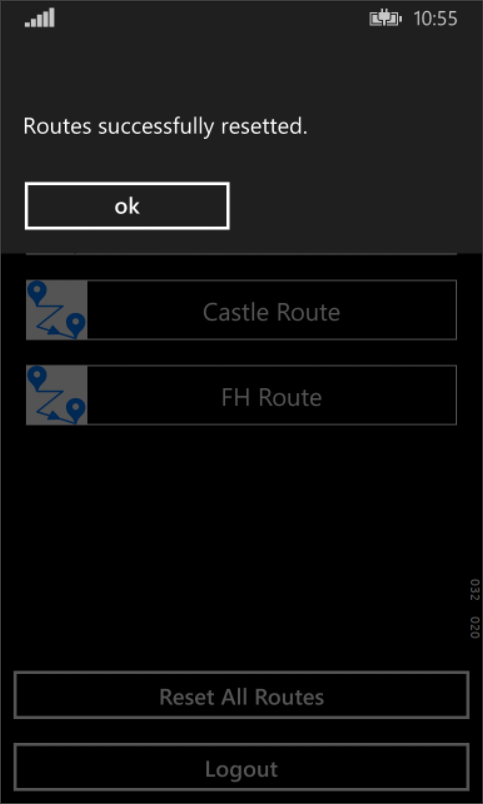
\includegraphics[width=.95\textwidth]{images/routePage_ResetRoutes}
\caption{Zurücksetzen aller Routen}
\end{figure}

\subsection{Details einer Route}

\begin{figure}[h]
\centering
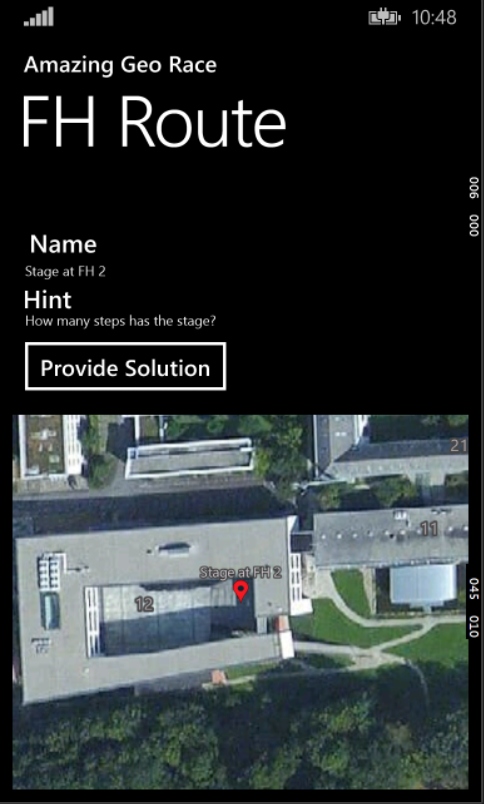
\includegraphics[width=.95\textwidth]{images/routeDetailsPage}
\caption{Details der gewählten Route mit Karte}
\end{figure}

\begin{figure}[h]
\centering
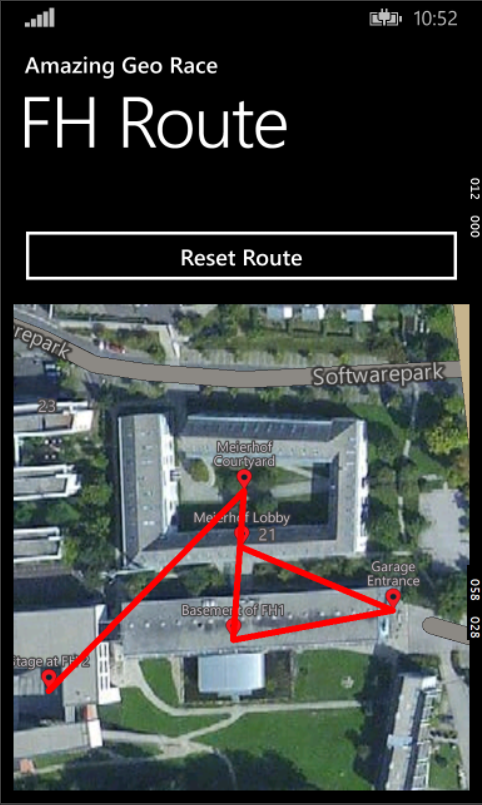
\includegraphics[width=.95\textwidth]{images/routeDetailsPage_Final}
\caption{Gelöste Route mit Karte}
\end{figure}
\begin{figure}[h]
\centering
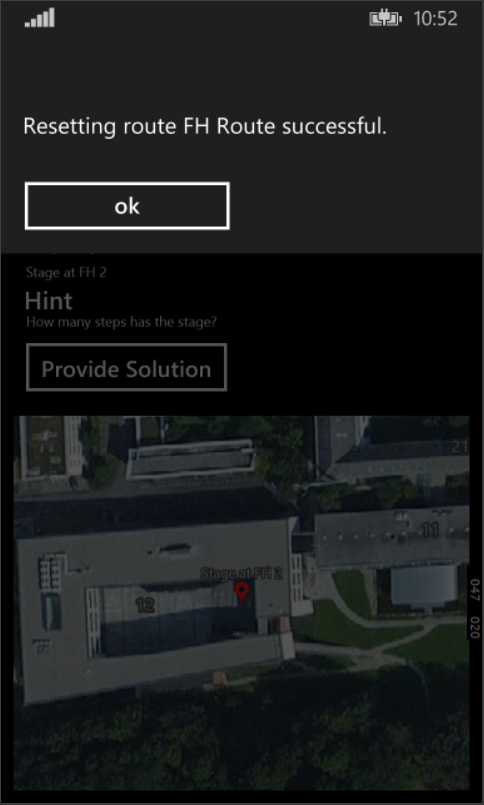
\includegraphics[width=.95\textwidth]{images/routeDetailsPage_Resetting}
\caption{Zurücksetzen einer Route}
\end{figure}

\subsection{Lösungen für Freischaltung}
\begin{figure}[h]
\centering
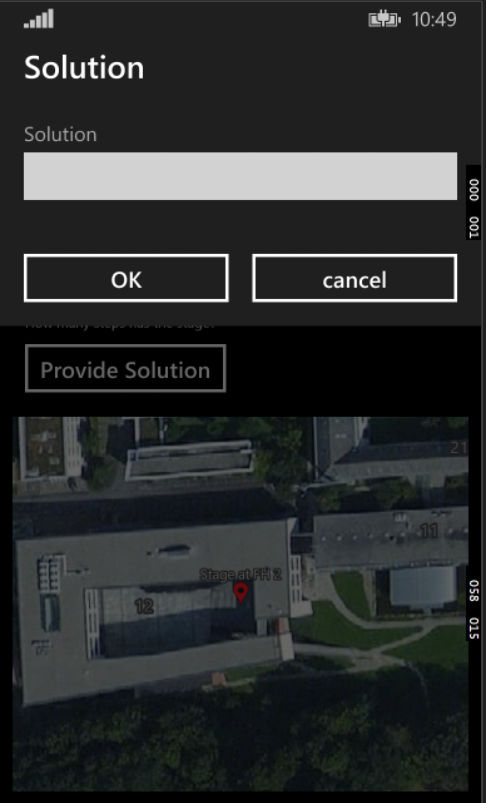
\includegraphics[width=.95\textwidth]{images/routeSolutionPage}
\caption{Ansicht des Lösungsdialogs}
\end{figure}
\begin{figure}[h]
\centering
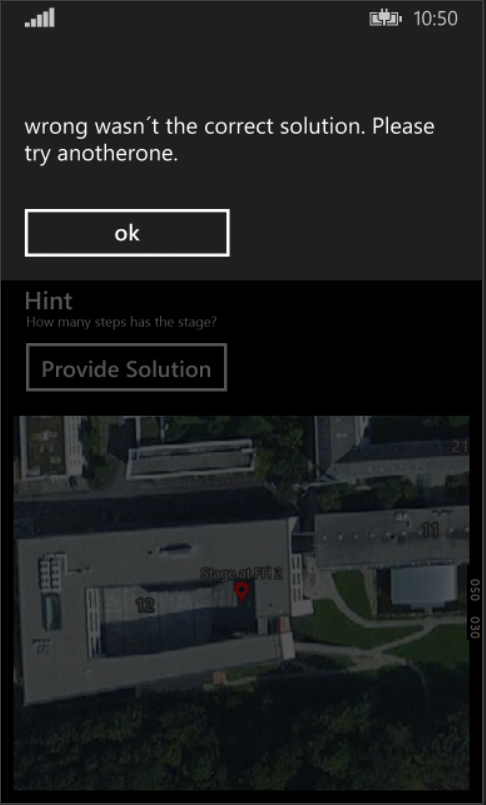
\includegraphics[width=.95\textwidth]{images/routeSolutionPage_Failed}
\caption{Falsche Lösung angegeben}
\end{figure}
\begin{figure}[h]
\centering
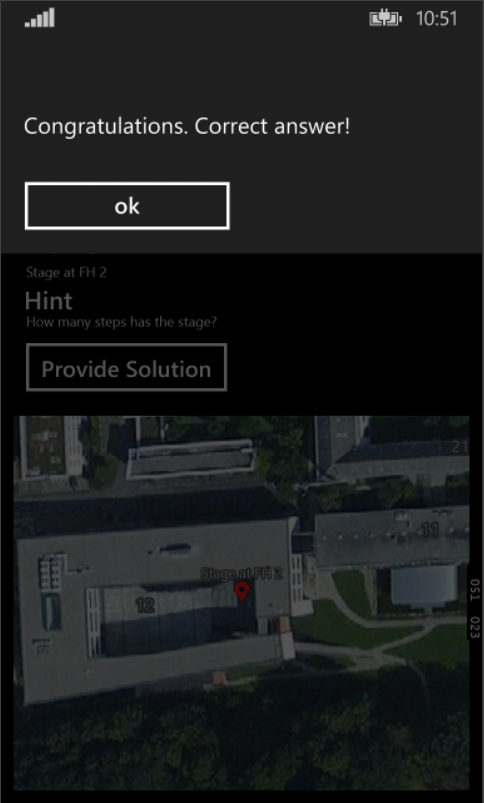
\includegraphics[width=.95\textwidth]{images/routeSolutionPage_Success}
\caption{Lösung richtig}
\end{figure}
\begin{figure}[h]
	\centering
	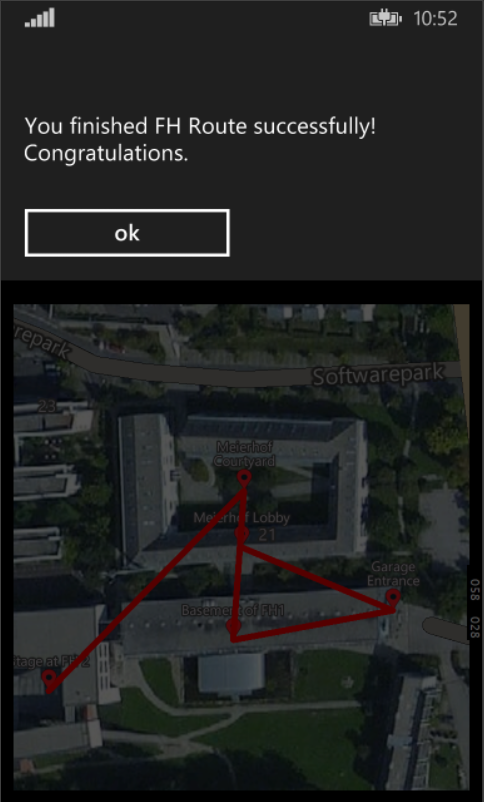
\includegraphics[width=.95\textwidth]{images/routeSolutionPage_Finished}
	\caption{Route erfolgreich abgeschlossen}
\end{figure}

\newpage
\section{Quellcode}

\subsection{Commands}
\lstinputlisting[caption=RelayCommand.cs]{../AmazingGeoRace/AmazingGeoRace/Commands/RelayCommand.cs}

\subsection{Common}
\lstinputlisting[caption=ExceptionHandling.cs]{../AmazingGeoRace/AmazingGeoRace/Common/ExceptionHandling.cs}
\lstinputlisting[caption=MessageBoxWrapper.cs]{../AmazingGeoRace/AmazingGeoRace/Common/MessageBoxWrapper.cs}
\lstinputlisting[caption=NavigationHelper.cs]{../AmazingGeoRace/AmazingGeoRace/Common/NavigationHelper.cs}
\lstinputlisting[caption=ObservableDictionary.cs]{../AmazingGeoRace/AmazingGeoRace/Common/ObservableDictionary.cs}
\lstinputlisting[caption=SuspensionManager.cs]{../AmazingGeoRace/AmazingGeoRace/Common/SuspensionManager.cs}

\subsection{Converters}
\lstinputlisting[caption=BooleanToCollapsedConverter.cs]{../AmazingGeoRace/AmazingGeoRace/Converters/BooleanToCollapsedConverter.cs}
\lstinputlisting[caption=BooleanToVisibilityConverter.cs]{../AmazingGeoRace/AmazingGeoRace/Converters/BooleanToVisibilityConverter.cs}

\subsection{Data}
\lstinputlisting[caption=WebService.cs]{../AmazingGeoRace/AmazingGeoRace/Data/WebService.cs}

\subsection{Domain}
\lstinputlisting[caption=LoginService.cs]{../AmazingGeoRace/AmazingGeoRace/Domain/LoginService.cs}
\lstinputlisting[caption=ServiceProxy.cs]{../AmazingGeoRace/AmazingGeoRace/Domain/ServiceProxy.cs}

\subsection{Models}
\lstinputlisting[caption=Checkpoint.cs]{../AmazingGeoRace/AmazingGeoRace/Models/Checkpoint.cs}
\lstinputlisting[caption=CheckpointRequest.cs]{../AmazingGeoRace/AmazingGeoRace/Models/CheckpointRequest.cs}
\lstinputlisting[caption=Request.cs]{../AmazingGeoRace/AmazingGeoRace/Models/Request.cs}
\lstinputlisting[caption=Route.cs]{../AmazingGeoRace/AmazingGeoRace/Models/Route.cs}
\lstinputlisting[caption=RouteRequest.cs]{../AmazingGeoRace/AmazingGeoRace/Models/RouteRequest.cs}

\subsection{ViewModels}
\lstinputlisting[caption=LoginViewModel.cs]{../AmazingGeoRace/AmazingGeoRace/ViewModels/LoginViewModel.cs}
\lstinputlisting[caption=MainViewModel.cs]{../AmazingGeoRace/AmazingGeoRace/ViewModels/MainViewModel.cs}
\lstinputlisting[caption=RaceDetailsViewModel.cs]{../AmazingGeoRace/AmazingGeoRace/ViewModels/RaceDetailsViewModel.cs}
\lstinputlisting[caption=ViewModelBase.cs]{../AmazingGeoRace/AmazingGeoRace/ViewModels/ViewModelBase.cs}

\subsection{Views-Markup}
\lstinputlisting[caption=LoginPage.xaml]{../AmazingGeoRace/AmazingGeoRace/Views/LoginPage.xaml}
\lstinputlisting[caption=MainPage.xaml]{../AmazingGeoRace/AmazingGeoRace/Views/MainPage.xaml}
\lstinputlisting[caption=RaceDetailsPage.xaml]{../AmazingGeoRace/AmazingGeoRace/Views/RaceDetailsPage.xaml}
\lstinputlisting[caption=SolutionDialog.xaml]{../AmazingGeoRace/AmazingGeoRace/Views/SolutionDialog.xaml}

\subsection{Views}
\lstinputlisting[caption=LoginPage.xaml.cs]{../AmazingGeoRace/AmazingGeoRace/Views/LoginPage.xaml.cs}
\lstinputlisting[caption=MainPage.xaml.cs]{../AmazingGeoRace/AmazingGeoRace/Views/MainPage.xaml.cs}
\lstinputlisting[caption=RaceDetailsPage.xaml.cs]{../AmazingGeoRace/AmazingGeoRace/Views/RaceDetailsPage.xaml.cs}
\lstinputlisting[caption=SolutionDialog.xaml.cs]{../AmazingGeoRace/AmazingGeoRace/Views/SolutionDialog.xaml.cs}

\subsection{App}
\lstinputlisting[caption=App.xaml]{../AmazingGeoRace/AmazingGeoRace/App.xaml}
\lstinputlisting[caption=App.xaml.cs]{../AmazingGeoRace/AmazingGeoRace/App.xaml.cs}

\end{document}